\section{System model}

\subsection{Scenarios}


\subsection{Use cases}

\title{Task Stealing (Nice to have)}

\begin{enumerate}[1. ]


\item Brief Description
\newline
This use case describes the way a task stealing algorithm works inside a dynamic scheduler in order to reduce the amount of process migration between processors.

\item Actors
\newline
No actors. 


\item Preconditions
\begin{enumerate}
\item The scheduler has been initialized and it has already created a MPI memory window for RMA (Remote Memory Access).
\item Information about initial tasks has been collected from code preprocessing, received tasks from which have been placed to the queue.
\end{enumerate}

\item Basic Flow of Event
\newline
The use case begins when the scheduler checks if there are tasks in its own queue.If there is a task in the queue, it will be executed. After the task has been executed, all collected results will get placed in the database in an organized manner.
If there isn't any task in the queue, the task stealing process will be initiated. First of all, the scheduler will cycle through all running processes in other processors and try to steal an idle task from them. In order to check the other processes' queue for an idle task, the scheduler tries to block the RMA window for offsets and statuses, after which it checks whether there are any idle tasks. If the queue is empty or if the RMA window is currently blocked, the scheduler repeats the same procedure for remaining processors. If after checking all processes, no idle task was found, the scheduler changes its own state to idle. If this idle state doesn't change for a specific amount of cycles, which means that no tasks were stolen in this period, the scheduler finally checks to make sure that no process is currently running in any processor and if that's the case, it finishes its own routine. 


\item Post-conditions
\begin{enumerate}
\item The scheduler frees the allocated MPI memory window for RMA.
\item The scheduler executes the finishing post processing routine, where it collects information from the whole process (e.g. global total run time).
\end{enumerate}

\item Special requirements

\begin{enumerate}
\item The scheduler should have access to the executer interface.
\item The scheduler should be accessible through an interface, in order to receive new tasks from the code interface.
\end{enumerate}

\end{enumerate}

\subsection{Object model}
\title{Basic module diagram}
\newline
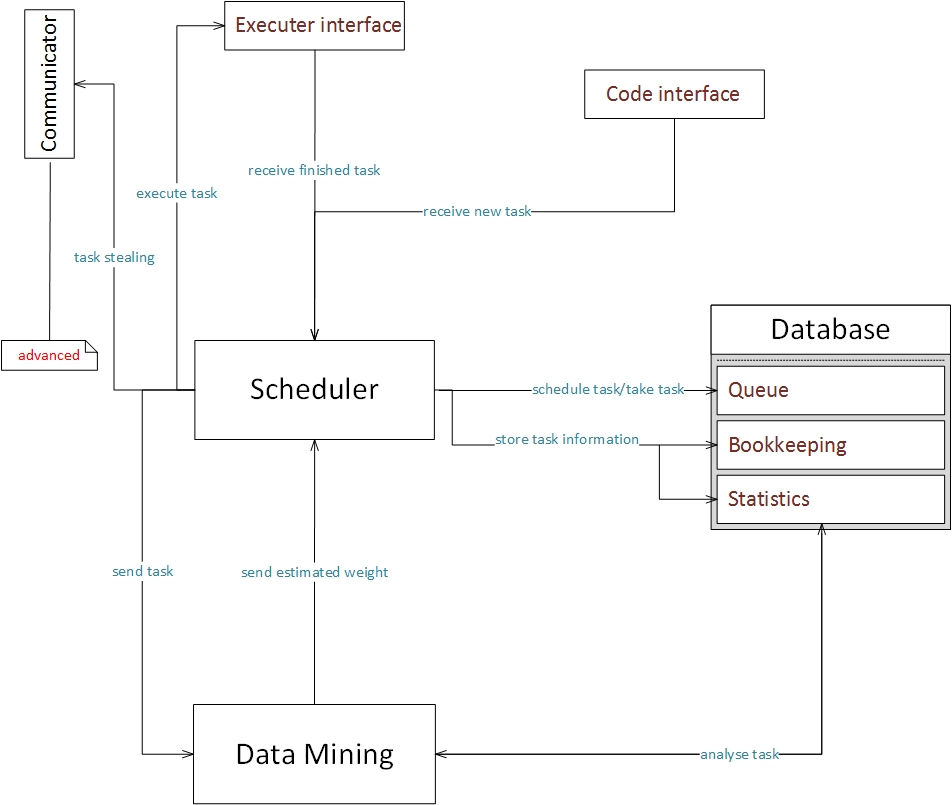
\includegraphics[width=15cm]{images/modules.jpg}
\newpage
\subsection{Dynamic models}

\begin{itemize}
\item Sequence diagram \newline
	\begin{figure}
	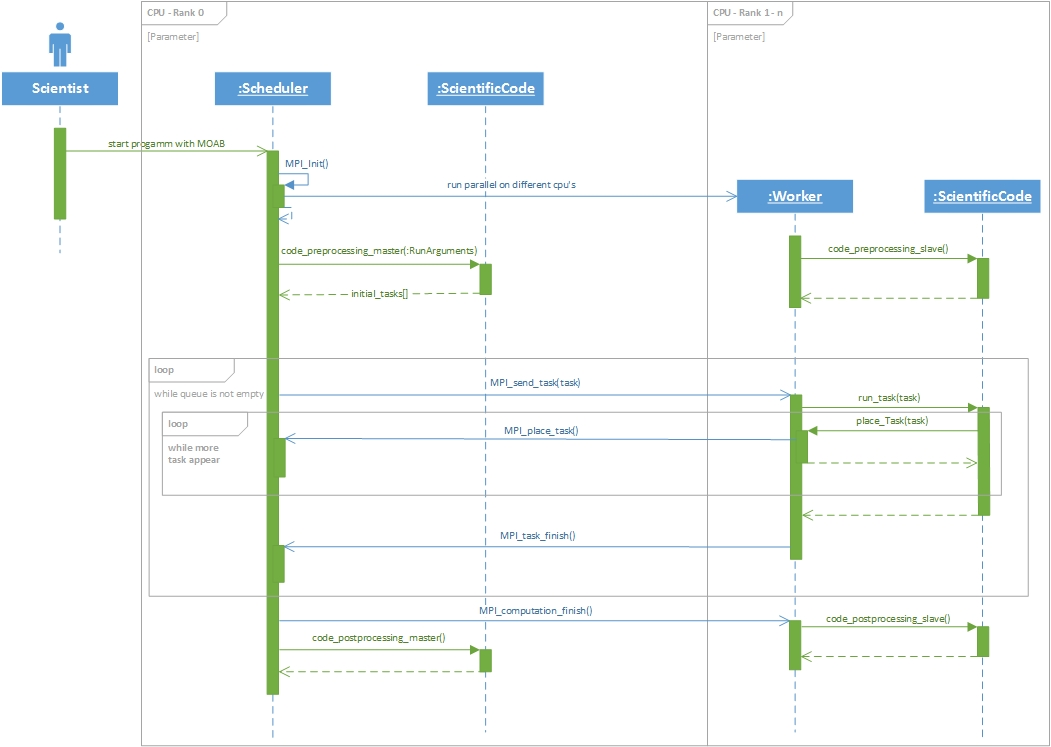
\includegraphics[width=15cm]{images/Master-slave.jpg}
	\caption{Master-slave diagram} 
	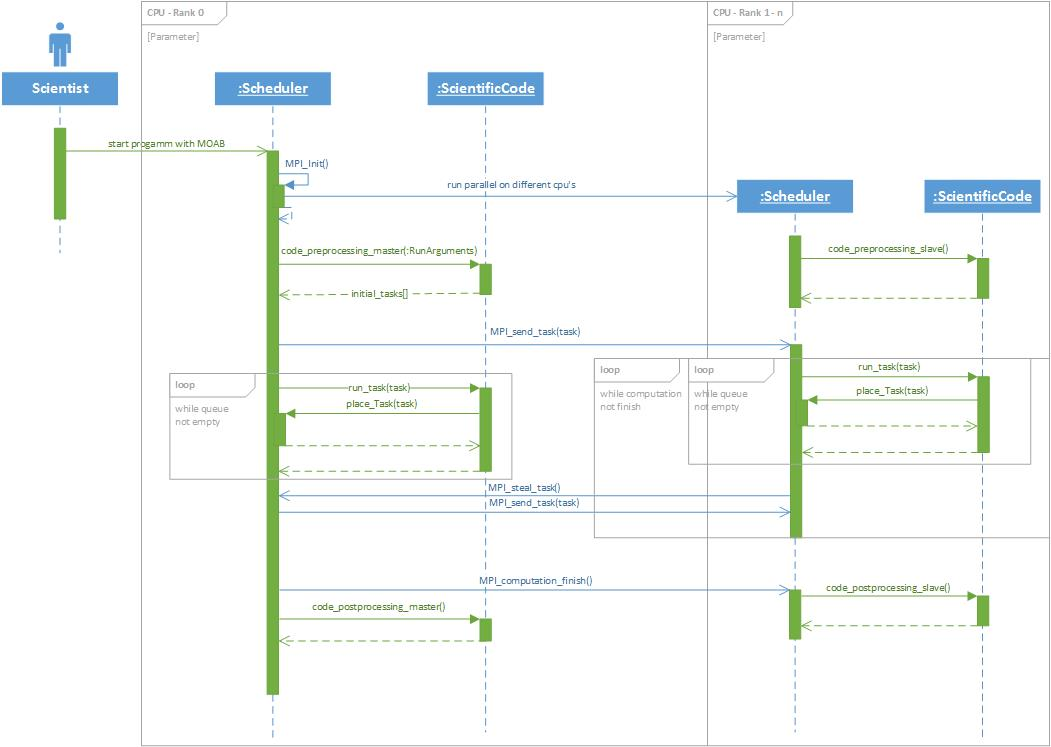
\includegraphics[width=15cm]{images/Task-stealing.jpg}
	\caption{Task-stealing algorithm}
	\end{figure}
\end{itemize}
\subsection{Graphical user interface}
